\documentclass[12pt]{beamer}
\usepackage{subcaption}
\usepackage[magyar]{babel}
\usepackage{t1enc}
\usepackage{tikz}
\usepackage{xcolor}
\usepackage{pgfplots}
\pgfplotsset{compat=1.18}
\usetheme{Berkeley}
\usecolortheme{default}
\definecolor{maroon}{rgb}{0.5, 0.0, 0.0}
\definecolor{mathgreen}{HTML}{509600}

%\setbeamercovered Nincs rá szükségünk
%\newtheorem{tetel}{Tétel}

\begin{document}
	\author{Szabó András \& Sándor Máté}
	\title{tikz \& pgfplots}
	%\subtitle{Bevezetés a \TeX-be} Nincs rá szükségünk
	\date{2021/22/I.\ félév}
	\institute{Miskolci Egyetem Sztárképző}
	\frame[plain]{\maketitle}
	
	%tableofcontent nem kell nekünk
	
	%Egyenletek létrehozása a Tikz és Pgfplots segítségével
	
		
	
	\section{Paragrafusok}

		\begin{frame}{TXT beolvasás}
			\includegraphics[height=7cm]{adat.png}
		\end{frame}
	
	
	\subsection{Paragrafus txt-ből}
	\begin{frame}{Paragrafus txt-ből}
		\begin{columns}[T] % align columns
			\begin{column}{.48\textwidth}
				{\color{gray}
				
				{\huge PDF Nézet}
				
				\rule{\linewidth}{3pt}}
				
				\begin{tikzpicture}[scale=0.50]
					\begin{axis}[
						title={\LARGE TXT Paragrafus},
						xlabel={$x$},
						ylabel={$y$},
						]
						\addplot[blue]table {adat.txt};
					\end{axis}
				\end{tikzpicture}
				
				
			\end{column}%
			\hfill%
			\begin{column}{.48\textwidth}
				{\color{blue}
				
				{\huge \TeX \! Kód}
				
				\rule{\linewidth}{3pt}}
				
				{\color{cyan}\textbackslash begin\{{\color{blue}tikzpicture}\}
				
					{\color{maroon}\quad {\color{orange} \textbackslash begin}\{axis\}[
					
						title=TXT Paragrafus,
						
						xlabel={{\color{mathgreen}\$x\$}},
						
						ylabel={{\color{mathgreen}\$y\$}},]
						
						{\color{orange}\textbackslash addplot}[blue]table \{adat.txt\};
						
					{\color{orange}\quad\textbackslash end}\{axis\}
					
				\textbackslash end\{{\color{blue}tikzpicture}\}}}
				
				
			\end{column}%
		\end{columns}
	\end{frame}

	\subsection{Négyzetfüggvény}
		\begin{frame}{Négyzetfüggvény}
		\begin{columns}[T] % align columns
			\begin{column}{.48\textwidth}
				\color{gray}
				
				{\huge PDF Nézet}
				
				\rule{\linewidth}{3pt}
				
			 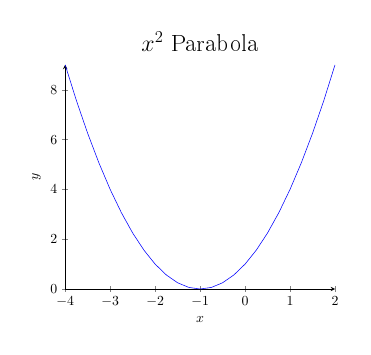
\begin{tikzpicture}[scale=0.50]
				\begin{axis}[
					title={\LARGE $x^2$ Parabola},
					xlabel={$x$},
					ylabel={$y$},
					axis lines = left,
					yticklabel pos=upper,
					xticklabel pos=upper,
					]
					\addplot[blue,domain=-4:2] {(x+1)^2};
				\end{axis}
			\end{tikzpicture}
				
				
			\end{column}%
			\hfill%
			\begin{column}{.48\textwidth}
				{\color{blue}
					
					{\huge \TeX \! Kód}
					
					\rule{\linewidth}{3pt}}
				
				{\color{cyan}\textbackslash begin\{{\color{blue}tikzpicture}\}
					
					{\color{maroon}\quad {\color{orange} \textbackslash begin}\{axis\}[
						
						title={{\color{mathgreen}\$x \^\ 2\$}},
						
						xlabel={{\color{mathgreen}\$x\$}},
						
						ylabel={{\color{mathgreen}\$y\$}},
						
						axis lines = left
						
						xticklabel pos=upper,
						yticklabel pos=upper,]
												
						{\color{orange}\textbackslash addplot}[blue,domain=\\-4:2] \{(x+1) \^\ 2\};
						
						{\color{orange}\quad\textbackslash end}\{axis\}
						
						\textbackslash end\{{\color{blue}tikzpicture}\}}}
				
				
			\end{column}%
		\end{columns}
 	\end{frame}

	\subsection{Több függvény egy ábrán}
	\begin{frame}{Több függvény egy ábrán}
		\begin{columns}[T] % align columns
			\begin{column}{.48\textwidth}
				\color{gray}
				
				{\huge PDF Nézet}
				
				\rule{\linewidth}{3pt}
				
				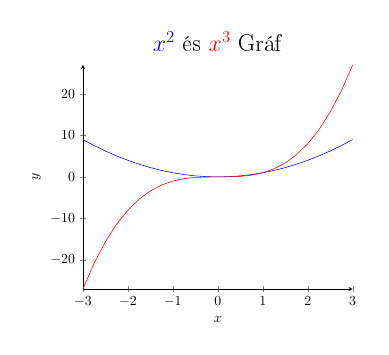
\begin{tikzpicture}[scale=0.50]
					\begin{axis}[
						title={\LARGE {\color{blue}$x^2$} és {\color{red}$x^3$} Gráf},
						xlabel={$x$},
						ylabel={$y$},
						axis lines = left,
						yticklabel pos=upper,
						xticklabel pos=upper,
						]
						\addplot[blue,domain=-3:3] {x^2};
						\addplot[red,domain=-3:3] {x^3};
					\end{axis}
				\end{tikzpicture}
				
				
			\end{column}%
			\hfill%
			\begin{column}{.48\textwidth}
				{\color{blue}
				
				{\huge \TeX \! Kód}
				
				\rule{\linewidth}{3pt}}
			
		{\scriptsize{}{\color{cyan}\textbackslash begin\{{\color{blue}tikzpicture}\}
				
				{\color{maroon}\quad {\color{orange} \textbackslash begin}\{axis\}[
					
					title={{\color{mathgreen}\$x \^\ 2\$}},
					
					xlabel={{\color{mathgreen}\$x\$}},
					
					ylabel={{\color{mathgreen}\$y\$}},
					
					{\quad yticklabel axis line = left,}
					{\quad yticklabel pos=upper,}
					{\quad xticklabel pos=upper,}]
					
					{\color{orange}\textbackslash addplot}[blue,domain=-3:3] \{x \^\ 2\};
					{\color{orange}\textbackslash addplot}[red,domain=-3:3] \{x \^\ 3\};
					
					{\color{orange}\quad\textbackslash end}\{axis\}
					
					\textbackslash end\{{\color{blue}tikzpicture}\}}}}
				
				
			\end{column}%
		\end{columns}
	\end{frame}
	
		\subsection{Sin(x) függvény}
		\begin{frame}{Sin(x) függvény}
			\begin{columns}[T] % align columns
				\begin{column}{.48\textwidth}
					\color{gray}
					
					{\huge PDF Nézet}
					
					\rule{\linewidth}{3pt}
					
					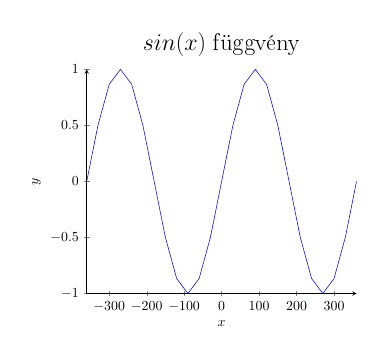
\begin{tikzpicture}[scale=0.50]
						\begin{axis}[
							title={\LARGE $sin(x)$ függvény},
							xlabel={$x$},
							ylabel={$y$},
							axis lines = left,
							yticklabel pos=upper,
							xticklabel pos=upper,
							]
							\addplot[blue,domain=-360:360] {sin(x)};
						\end{axis}
					\end{tikzpicture}
					
					
				\end{column}%
				\hfill%
				\begin{column}{.48\textwidth}
					{\color{blue}
						
						{\huge \TeX \! Kód}
						
						\rule{\linewidth}{3pt}}
					
					{\footnotesize{\color{cyan}\textbackslash begin\{{\color{blue}tikzpicture}\}
							
							{\color{maroon}\quad {\color{orange} \textbackslash begin}\{axis\}[
								
								{\quad axis lines=left,}
								
								{\quad yticklabel pos=upper,}
								
								{\quad xticklabel pos=upper,}
								]}
							{\quad \color{orange}\textbackslash addplot}[blue,domain=\{\quad -360:360] {sin(x)};}
						
						{\color{orange}\quad\textbackslash end}\{axis\}
						
						\textbackslash end\{{\color{blue}tikzpicture}}\}
			
			
		\end{column}%
	\end{columns}
	\end{frame}
	
	\subsection{Jelmagyarázat}
	\begin{frame}{Jelmagyarázat}
		\begin{columns}[T] % align columns
			\begin{column}{.48\textwidth}
				\color{gray}
				
				{\huge PDF Nézet}
				
				\rule{\linewidth}{3pt}
				
				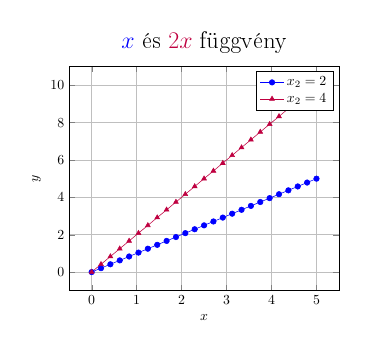
\begin{tikzpicture}[scale=0.50]
					\begin{axis}[
						title={\LARGE {\color{blue}$x$} és {\color{purple}$2x$} függvény},
						xlabel={$x$},
						ylabel={$y$},
						grid=major,
						legend entries={$x_2=2$,$x_2=4$}
						]
						\addplot[blue,domain=0:5,mark=*] {x};
						\addplot[purple,domain=0:5,mark=triangle*] {2*x};
					\end{axis}
				\end{tikzpicture}
				
				
			\end{column}%
			\hfill%
			\begin{column}{.48\textwidth}
				{\color{blue}
					
					{\huge \TeX \! Kód}
					
					\rule{\linewidth}{3pt}}
				
				{\scriptsize{\color{cyan}\textbackslash begin\{{\color{blue}tikzpicture}\}
						
						{\color{maroon}\quad {\color{orange} \textbackslash begin}\{axis\}[
							
							
							{\quad grid=major}
							
							{\quad legend entries={\$x\_2=2\$, \\ \quad \$x\_2=4\$}}
							\\{\quad ]}\\
							{\quad \color{orange}\textbackslash addplot}[blue,domain=\\{\quad 0:5,mark=*] \{x\};}
							
							{\quad \color{orange}\textbackslash addplot}[blue,domain=\\{\quad 0:5,triangle*] \{2x\};}
							
							{\color{orange}\quad\textbackslash end}\{axis\}
							
							\textbackslash end\{{\color{blue}tikzpicture}\}}}}
				
				
			\end{column}%
		\end{columns}
	\end{frame}

	
\end{document}